
%%%%%%%%%%%%%%%%%%%%%%% file typeinst.tex %%%%%%%%%%%%%%%%%%%%%%%%%
%
% This is the LaTeX source for the instructions to authors using
% the LaTeX document class 'llncs.cls' for contributions to
% the Lecture Notes in Computer Sciences series.
% http://www.springer.com/lncs       Springer Heidelberg 2006/05/04
%
% It may be used as a template for your own input - copy it
% to a new file with a new name and use it as the basis
% for your article.
%
% NB: the document class 'llncs' has its own and detailed documentation, see
% ftp://ftp.springer.de/data/pubftp/pub/tex/latex/llncs/latex2e/llncsdoc.pdf
%
%%%%%%%%%%%%%%%%%%%%%%%%%%%%%%%%%%%%%%%%%%%%%%%%%%%%%%%%%%%%%%%%%%%


\documentclass[runningheads,a4paper]{llncs}

\usepackage{amssymb}
\usepackage{amsmath}
\setcounter{tocdepth}{3}
\usepackage{graphicx}
\newtheorem{mydef}{Definition}
\newtheorem{mylemma}{Lemma}
\usepackage{algorithm}
\usepackage{tabularx}

\usepackage[noend]{algpseudocode}


\usepackage{url}
\urldef{\mailsa}\path|{jayg, cmhill, mpop}@cs.umd.edu|    
\newcommand{\keywords}[1]{\par\addvspace\baselineskip
\noindent\keywordname\enspace\ignorespaces#1}

\begin{document}

\mainmatter  % start of an individual contribution

% first the title is needed
\title{Identifying Inter-Genomic Repeats Using Fast, Approximate Methods for Betweenness Centrality}

% a short form should be given in case it is too long for the running head
\titlerunning{Inter-Genomic Repeats Using Betweenness Centrality}

% the name(s) of the author(s) follow(s) next
%
% NB: Chinese authors should write their first names(s) in front of
% their surnames. This ensures that the names appear correctly in
% the running heads and the author index.
%
\author{Jay Ghurye%
\and Christopher M. Hill\and Mihai Pop}
%
\authorrunning{Ghurye et al.}
% (feature abused for this document to repeat the title also on left hand pages)

% the affiliations are given next; don't give your e-mail address
% unless you accept that it will be published
\institute{University of Maryland, College Park\\
\mailsa\\}

%
% NB: a more complex sample for affiliations and the mapping to the
% corresponding authors can be found in the file "llncs.dem"
% (search for the string "\mainmatter" where a contribution starts).
% "llncs.dem" accompanies the document class "llncs.cls".
%

\toctitle{Lecture Notes in Computer Science}
\tocauthor{Authors' Instructions}
\maketitle


\begin{abstract}
Genomic repeats are the most important challenge in genomic assembly. While for single genomes the effect of repeats is largely addressed by modern long-read sequencing technologies, in metagenomic data intra-genome and, more importantly, inter-genome repeats continue to be a significant impediment to effective genome reconstruction.  Detecting repeats in metagenomic samples is complicated by characteristic features of these data, primarily uneven depths of coverage and the presence of genomic polymorphisms.  The scaffolder Bambus 2 introduced a new strategy for repeat detection based on the betweenness centrality measure -- a concept originally used in social network analysis. The exact computation of the betweenness centrality measure is, however, computationally intensive and impractical in large metagenomic datasets.  Here we explore the effectiveness of approximate algorithms for network centrality to accurately detect genomic repeats within metagenomic samples.  We show that approximate measures of centrality achieve much higher computational efficiencies with a minimal loss in the accuracy of detecting repeats in metagenomic data.  
\keywords{Metagenomics, Algorithms, Centrality, Graph}
\end{abstract}


\section{Introduction}

Genomic repeats are the most important challenge in genomic assembly even for isolate genomes.  When reads are shorter than the repeats (a common situation until the recent development of long read sequencing technologies) it can be shown that the number of genome reconstructions consistent with the read data grows exponentially with the number of repeats~\cite{kingsford}.  The use of additional information to constrain the one genome reconstruction representing the actual genome being assembled leads to computationally intractable problems. In other words, when reads are shorter than repeats the correct and complete reconstruction of a genome is impossible.  In the case of isolate genomes, long read technologies have largely addressed this challenge, at least for bacteria where the majority of genomic repeats fall within the range of achievable read lengths~\cite{koren2015one}.  In metagenomics, however, the problem is compounded by the fact that microbial mixtures often include multiple closely-related genomes differing in just a few locations.  The genomic segments shared by closely related organisms -- inter-genomic repeats -- are substantially larger than intra-genomic repeats and cannot be fully resolved even if long read data were available. Instead, the best hope is to identify and flag these repeats  in order to avoid mis-assemblies that incorrectly span across genomes. 

Repeat detection strategies have been employed in genome assembly from the early days of the field, and numerous approaches have been developed for this purpose.  In metagenomics, however, the problem is exacerbated by uneven coverage across contigs and by the fact that both inter- and intra-genomic repeats exist in the data, factors impacting statistical approaches for repeat detection.  An alternate approach based on the social network concept of betweenness centrality was introduced in Bambus 2~\cite{bambus}. An example of the effectiveness of this approach in a simple community composed of two genomes is shown in Fig.~\ref{fig:es_mix}.   The full implementation of betweenness centrality requires an all-pairs shortest path computation which is computationally too intensive for typical metagtenomic datasets.  In Bambus 2, for example, repeat finding in a typical stool sample requires days of computation.
To overcome this limitation, we explore the use of parallel and approximate betweenness centrality algorithms for repeat detection in metagenomic assembly graphs, and the effect of the level of approximation on the efficiency and accuracy of these algorithms.  

\begin{figure*}[htbp]
\centering
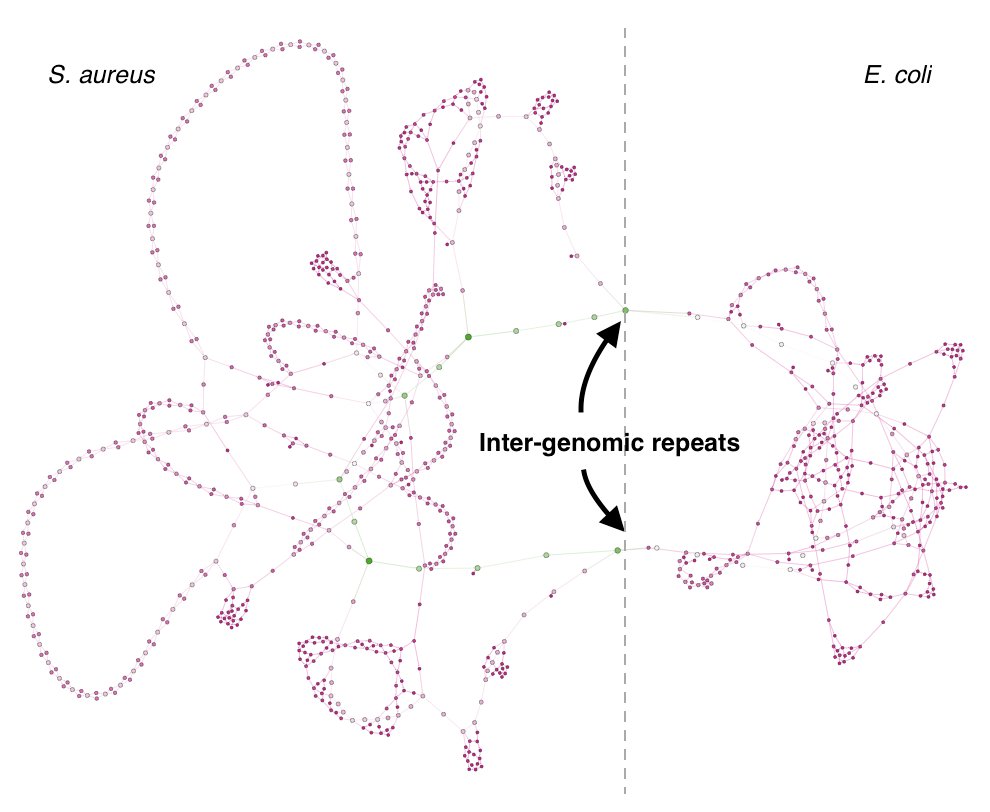
\includegraphics[width=0.70\textwidth]{es_mix_200kb_k21.png}
\caption{Assembly graph of a simulated community consisting of 200 Kbp subsets of \textit{Escherichia coli} str. K-12 MG1655 and \textit{Staphylococcus aureus}.  Nodes are colored and sized based on their relative betweenness centrality with larger, green nodes indicating a higher centrality. The highlighted nodes are inter-genomic repeats whose deletion would separate the graph. Note that the betweenness centrality measure correctly identifies these nodes.}
\label{fig:es_mix}
\end{figure*}

\section{Related Work}

\subsection*{Betweenness Centrality}
In network analysis, metrics of centrality are used to identify the most important nodes within a graph. Several metrics to measure centrality have been proposed, but in this work, we use betweenness centrality. The betweenness centrality of a particular node is equal to the number of shortest paths from all nodes to all others that pass through that node. Intuitively, a node that is frequently found on paths connecting other nodes is ``important''.  In assembly, we can likewise infer that nodes that are on the paths connecting multiple distinct segments of a genomic assembly likely represent repetitive sequences.  Formally, for a node $v$, centrality is defined by following expression:

$$g(v) = \sum_{s \neq t \neq v} \frac{\sigma_{st}(v)}{\sigma_{st}}$$

where $\sigma_{st}$ is the total number of shortest paths from node $s$ to node $t$ and $\sigma_{st}(v)$ is the number of those paths passing through $v$.

Brandes\cite{brandes} gives an exact algorithm for computing betweenness centrality of all the nodes that is based on solving a single-source shortest path (SSSP) problem for each node. A SSSP computation from $s$ produces a directed acyclic graph (DAG) encoding all shortest paths starting at $s$. The contributions of these paths to the betweenness counters can be computed in linear time using backward aggregation. Brandes' algorithm calculates $\sigma_{st}$  simultaneously with the shortest path calculations: $\sigma_{ss} = 1$ and for $s \neq t, \sigma_{st} = \sum_{v \in pred(t)} \sigma_{sv}$ where $pred(t)$ is a collection of the immediate predecessors of  $t$ on every shortes path ending at $t$. In a subsequent aggregation phase, nodes are processed by non-decreasing distance from $s$. So we have: 
$$\delta_{s}(v) = \sum_{w \in succ(v)} \frac{\sigma_{sv}}{\sigma_{sw}}(1+\delta_{s}(w))$$

where $\delta_{s}(v) = \frac{\sigma_{st}(v)}{\sigma_{st}}$ and $succ(v)$ is an immediate successor of $v$  in the shortest path DAG.   
This algorithm takes time $\Theta(mn)$ for unit edge weight graphs and $\Theta(mn + n^{2}log(n))$ for weighted graphs. This algorithm does not scale well in large networks with millions of nodes and edges. Bader and Madduri\cite{bader} provide a massively parallel implementation of the exact algorithm, but even the parallel implementation only scales in practice to  a few million nodes, limiting its application to larger metagenomic assembly graphs.

\subsection*{Approximate Betweenness Centrality Based on Node Sampling}
Due to scalability limitations of exact betweenness centrality, several approximation algorithms for betweenness centrality have been proposed. Bader and Pich\cite{bp} provide an approximation algorithm by choosing a subset of $k$ starting nodes called pivots and apply the Brandes algorithm to just the chosen nodes. This algorithm was shown to overestimate the centrality of some unimportant nodes which are close to the pivots. Geisberger et al. \cite{sanders} sole this issue by changing the scheme for aggregating betweenness contributions so that nodes close to the pivots are not unduly profited. The algorithm starts with the sample of $k$ nodes from $|V| = n$ nodes in graph. In each iteration, it chooses one of $2n$ shortest path at random. Here there are $2n$ sample shortest paths because the algorithm can perform a forward search from $s \in V$ or a backward search from $t \in V$ and each $s$ and $t$ can have $n$ values. Let $\delta_{P}(v)$ be the contribution received by node $v$ due to shortest path $P$. It can be shown that \cite{sanders} due to all shortest paths $P$ on which $v$ lies, $v$ receives contribution 

$$\delta(v) := \delta_{s}(v) := \sum_{t \in V}\sum \{\delta_{P}(v):  P \in SP_{st}(v)\}$$
due to a forward search, and 

$$\delta(v) := \delta_{t}(v) := \sum_{s \in V}\sum \{\delta_{P}(v):  P \in SP_{st}(v)\}$$
due to a backward search. 

The runtime and accuracy of these algorithms depend on the number of nodes sampled from the graph.

\subsection*{Approximate Betweenness Centrality Based on Sampling Shortest Paths}
A different approximation strategy was proposed by Matteo et al. \cite{matteo} based on randomized sampling of shortest paths (rather than nodes), approach which offers probabilistic guarantees on the quality of approximation. This algorithm guarantees that all approximate values of betweenness for all vertices are within an additive factor $\epsilon \in (0,1)$ from the real values with probability at least $1-\delta$. To derive bounds on sample size, results from VC dimension theory\cite{vc} are used. The main advantage of this algorithm is that the sample size does not depend on the size of the graph, but only on the maximum number vertices in a shortest path, measure called the \textit{vertex diameter} of the graph. The sample size $r$ of shortest paths is found out with the help of $VD(G)$ as follows:
$$
r = \frac{c}{\epsilon^{2}}(\left\lfloor{log_{2}(VD(G) - 2)}\right\rfloor + 1 + ln\frac{1}{\delta})
$$ 
where $c$ is a constant with value $0.5$. 

The algorithm estimates the vertex diameter of the graph using a simple $2-$approximation algorithm. The shortest paths are sampled using weighted random sampling. The runtime of this algorithm is dominated by the computation of shortest path at each step which takes time $O(|V| + |E|)$ for unweighted graphs (BFS) and $O(|E| + |V|log|V|)$ otherwise (Dijkstra's algorithm). This value is multiplied by the number of iterations to obtain the final complexity.


\section{Methods}


\subsection*{Metagenomic Data}

We evaluate the efficacy of detecting inter-genomic repeats using the approximate betweenness centrality methods on simulated metagenomic assembly graphs.
We start with a collection of genomes from which we construct idealized De Bruijn graphs (assuming perfect coverage and no sequencing errors). Next we modify the De Bruijn graph generated from the collection of genomes to identify repeats $>=k$. We define \textit{unipaths} as maximal paths comprising nodes with in- and out-degrees equal to $1$. We compress all the unipaths into single nodes representing the concatenated labels of the collapsed nodes. 
The nodes in the resulting graph represent uniquely resolvable sequences of length $\geq k$.

We simulated metagenomic assembly graphs consisting of two, five, and ten bacterial genomes.
The composition of each simulated sample is described in Table \ref{tab:composition}.
For the five and ten metagenome samples, random bacterial genomes were chosen from the data set provided by \cite{shakya2013comparative}.
A $k$-mer size of 55 was chosen for the initial creation of the De Bruijn graph.

\begin{table}[h]
\centering
\caption[]{Composition of simulated metagenomic assembly graph.}
\begin{tabularx}{\linewidth}{|l|X|l|l|}
\hline
\textbf{Name} & \textbf{Genomes} & \textbf{Nodes} & \textbf{Edges} \\
\hline
2-genome & \textit{Escherichia coli} str. K-12, \textit{Staphylococcus aureus}  & 3,384 & 4,534 \\
\hline
5-genome & \textit{Burkholderia xenovorans} LB400, \textit{Archaeoglobus fulgidus} DSM 4304,  \textit{Pyrobaculum calidifontis} JCM 11548, \textit{Zymomonas mobilis subsp. mobilis} ZM4, \textit{Porphyromonas gingivalis} ATCC 33277 & 5,114 & 6,844  \\
\hline
10-genome  & \textit{Caldicellulosiruptor bescii} DSM 6725, \textit{Bacteroides vulgatus} ATCC 8482,
\textit{Bacteroides thetaiotaomicron} VPI-5482, \textit{Clostridium thermocellum} ATCC 27405,
\textit{Pyrobaculum arsenaticum} DSM 13514, \textit{Chlorobium phaeobacteroides} DSM 266,
\textit{Ruegeria pomeroyi} DSS-3, \textit{Treponema denticola} ATCC 35405,
\textit{Porphyromonas gingivalis} ATCC 33277, \textit{Nostoc sp.} PCC 7120  & 25,425 & 34,056\\
\hline
\end{tabularx}
\label{tab:composition}
\end{table}

In addition to the simulated metagenomic assembly graphs, we evaluate the runtimes of the two approximation algorithms for betweenness centrality on a human stool metagenomic sample. This graph has 3,797,425 nodes and 2,970,379 edges. We compared the runtime of Bambus2's repeat detection module on this data with the runtime of approximate betweenness centrality algorithms.  

\subsection*{Evaluation}
%We evaluate the effect of using approximation algorithms for betweenness centrality on finding inter-genome repeats using the simulated datasets described above.
%We use the notion of Sensitivity, specificity, and precision to define the quality of repeat detection.
A good repeat detection strategy should have high sensitivity, specificity, and precision. Sensitivity is the measure of proportion of actual repeats which are correctly identified by the algorithm. Specificity is the proportion of non-repeats correctly identified by the algorithm. Precision is the proportion of repeats identified that are correct. High sensitivity is desired because we want to remove as many repeats from the graph. High specificity is desired because we do not want to remove non-repeats which are incorrectly identified as repeats by algorithm. High precision helps us determine the usefulness of our methods. To calculate sensitivity, specificity, and precision, we define following terms:
\begin{itemize}
\item \textbf{True positives(TP):} Number of nodes marked as a repeat that is found within at least 2 genomes
\item \textbf{False positives(FP):} Number of nodes marked as a repeat that is only found within a single genome
\item \textbf{True negatives(TN):} Number of nodes marked as a non-repeat that is only found within a single genome
\item \textbf{False negatives(FN):} Number of nodes marked as a non-repeat that is found within at least 2 genomes
\end{itemize}

Using these quantities, we can define sensitivity and specificity as follows:
 $$Sensitivity = \frac{TP}{TP+FN}$$
 $$Specificity = \frac{TN}{TN+FP}$$
 $$Precision = \frac{TP}{TP + FP}$$

We evaluate the two approaches for calculating betweenness centrality based on sampling nodes and sampling shortest paths using the above measures.
For evaluating the effect of sampling nodes on inter-genomic repeat detection, we sample between 10 to 10,000 nodes per trial.
For evaluating shortest paths sampling, we select epsilon parameters between 0.01 and 0.20, corresponding to a level of error between $1\%$ and $20\%$.
We repeat each algorithm 10 times and report the averge results.


\subsection*{Cutoff Criteria For Identifying Repeats}
Centrality algorithms provide numeric estimates for the centrality of each node, values from which we can infer whether a graph node represents a repeat. In Bambus2~\cite{bambus} repeats were defined as nodes with a centrality score larger than three standard deviations from the mean centrality of the nodes in the graph. This strategy implicitly assumes the distribution of centrality values in the graph to follow a normal distribution.  We use the same definition here and also explore the use of an alternate statistic -- the  \textit{interquartile range(IQR)}. Let $Q_{1}$,$Q_{2}$, and $Q_{3}$ denote the lower, middle and upper quartiles respectively. IQR can be defined as the difference between the upper and lower quartile. So, $IQR = Q_{3} - Q_{1}$. To identify repeats we simply mark  all the nodes with centrality values larger than $Q_{3} + 1.5*IQR$. This latter approach no longer assumes that the centrality values are normally distributed. 

\subsection*{Implementation}
We investigate the performance of approximate betweenness centrality algorithms on the metagenomic assembly graphs using the implementations provided by \textsc{NetworKit}\cite{networkit} library. \textsc{NetworKit} contains efficient and parallel implementations of a collection of graph algorithms.
For our experiments, we use the parallelized implementation for the algorithm by Matteo et al.\cite{matteo} and serial implementation for the algorithm by Geisberger et al.\cite{sanders}.
We carried out all experiments on a 64-bit Linux machine with 12 CPUs and 50 GB memory. 

\section{Results} 


\subsection*{Approximate Betweenness Centrality Measures Increase Efficiency without a Significant Loss in Accuracy}

Across all datasets, the efficiency of the approach is correlated with the level of approximation for both node sampling and path sampling approaches (Figs. \ref{fig:sampled_nodes} and \ref{fig:sampled_paths}).  Accuracy is inversely proportional with the level of approximation.  The effectiveness of these methods is also higher in simpler communities.  In the 2-genome community,  all inter-genomic repeats were found by sampling as few as ten nodes, an order of magnitude less time than calculating the betweenness centrality using the full graph.  For the 5-genome graph, sampling as few as ten nodes yields a sensitivity of $86\%$ and full sensitivity is achieved with just 500 nodes, or approximately one tenth of the entire size of the assembly graph.  

The 10-genome graph is substantially more complex yielding much lower sensitivity for both node sampling and path sampling approaches.  The use of the inter-quartile range as a decision criterion improves the sensitivity from about $6\%$ to $35\%$ in the 10-genome graph at the cost of a reduction in specificity from $99.3\%$ to $90.9\%$.  Also, note that the path sampling approach is marginally more efficient than the node sampling procedure  - the worst runtime (at an error setting of $1\%$) is roughly equivalent to sampling about 1000 nodes.

\begin{figure}[htbp]
\centering
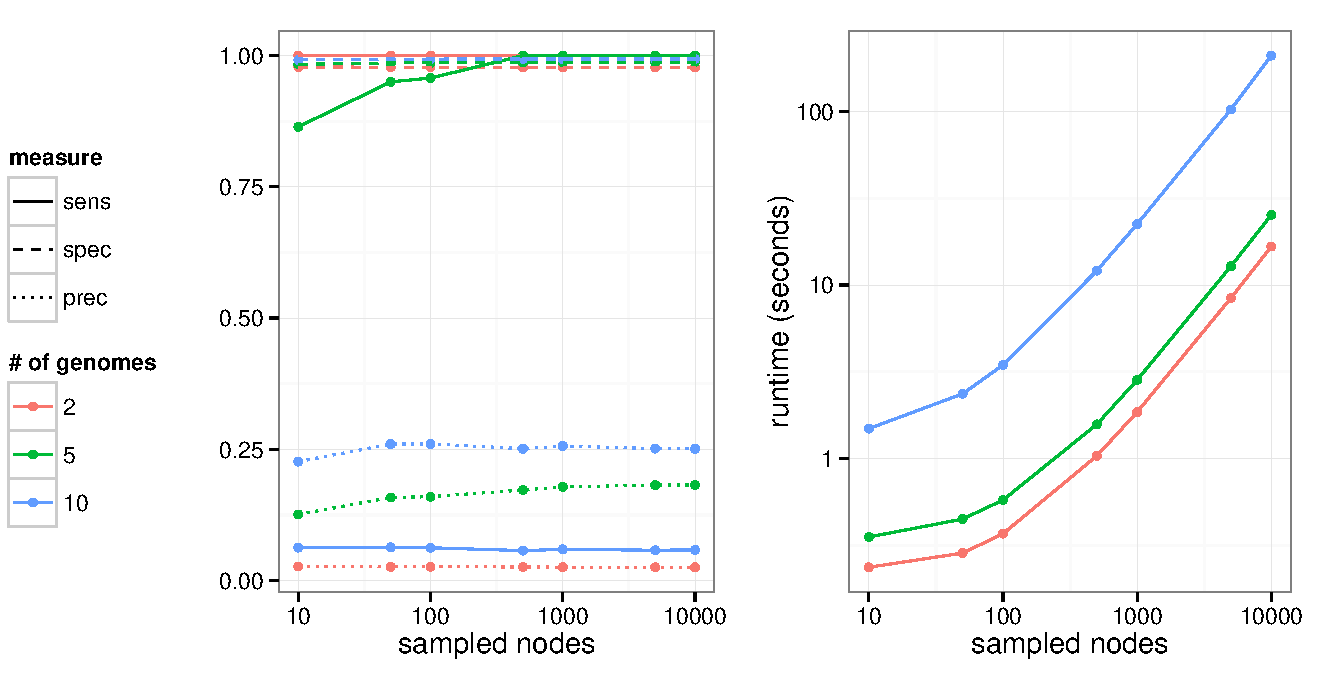
\includegraphics[width = \textwidth]{sampled_nodes}
\caption{Statistical measures of repeat detection quality for the simulated metagenomic assembly graphs. Betweenness centrality was approximated by randomly sampling nodes in the graph.}
\label{fig:sampled_nodes}
\end{figure}

\begin{figure}[htbp]
\centering
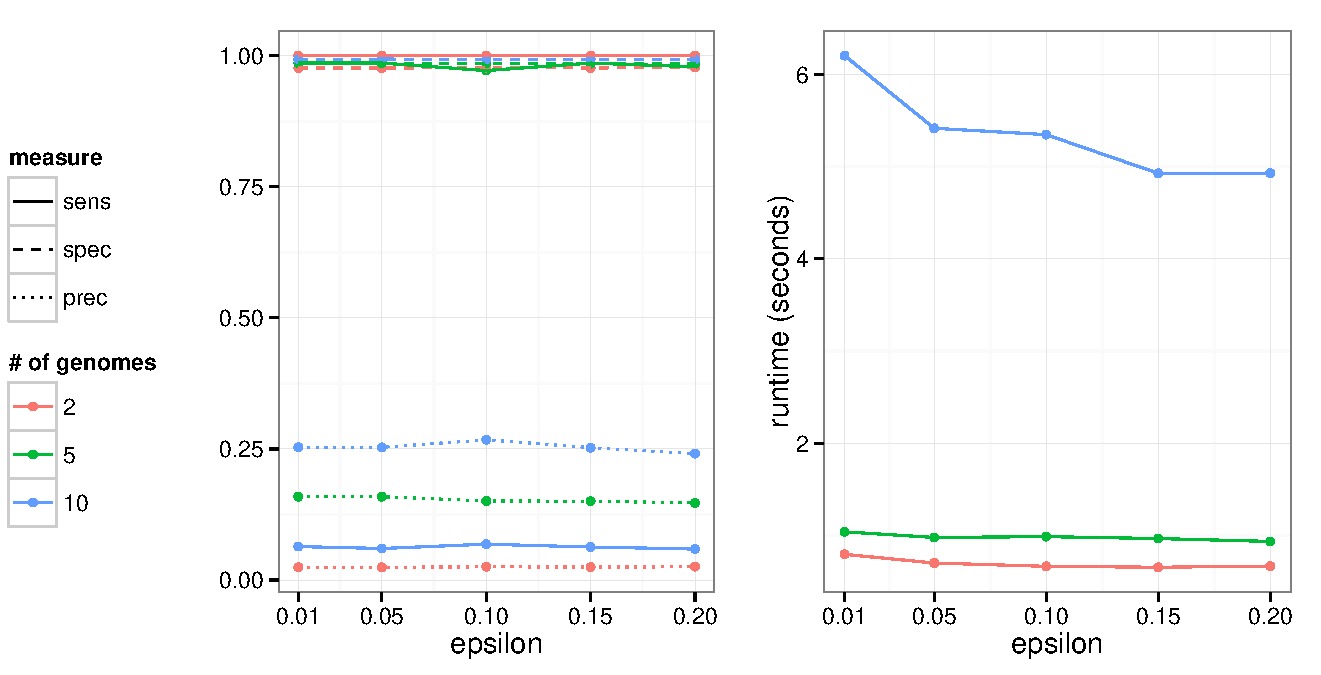
\includegraphics[width = \textwidth]{sampled_paths}
\caption{Statistical measures of repeat detection quality for the simulated metagenomic assembly graphs. Betweenness centrality was approximated within epsilon of their true value.}
\label{fig:sampled_paths}
\end{figure}


\subsection*{Results On Real Metagenomic Datasets}
We evaluated the performance of approximate betweenness centrality algorithms on an actual metagenomic stool sample and compared the runtime to that of the MarkRepeats procedure from Bambus 2.  On this dataset, comprising $3,797,425$ nodes and $2,970,379$ edges, Bambus 2 had not completed after 60 hours at which point we terminated the execution.  The path sampling approach with an error setting of $1\%$ ( $\epsilon = 0.1$) took $312.69$ seconds, while the node sampling approach toolk $469$ seconds for a $1,000$ node sample and 1.3 hours for a $10,000$  node sample.  


\section{Discussion}
Betweenness centrality is a proven method for finding inter-genomic repeats in metagenomic assemblies. The size of typical metagenomic assembly graphs often make it infeasible to calculate the exact betweenness centrality of each node, as demonstrated by the slow runtime of the MarkRepeats procedure from Bambus 2.  Here we have demonstrated the effectiveness of approximate measures of centrality able to identify repeats in a fraction of the time previously required.   We explored two alternative approximation strategies, based on node sampling and path sampling, respectively.  The runtime of node-sampling approaches can be more effectively estimated as it increases roughly linearly in the size of the sample selected.  Conversely, path sampling approaches can guarantee the level of approximation but runtime cannot be easily estimated. 

Despite promising results, our work has also revealed limitations of the approximate approaches - in the more complex communities the sensitivity of detection dropped significantly, though it was partly rescued by the use of a decision cut-off based on inter-quartile ranges.   We are currently exploring this phenomenon and whether it will have a significant impact on metagenomic assembly. It is likely that many of the repeats missed by the approximate procedure are small and local in nature and could be resolved through other means.  It is also possible that other approaches for outlier detection would be more effective in restoring the sensitivity of detection. 

\section{Conclusion}
Here we have demonstrated that approximate betweenness centrality approaches can be effectively used to detect repeats in metagenomic assemblies.  These approaches run in a fraction of the time needed to exactly compute betweenness centrality with only a small loss of accuracy in repeat detection. We currently plan to incorporate such algorithms in the Bambus scaffolding software in order to improve its efficiency, and also plan to further develop the repeat detection algorithms in order to improve their sensitivity in complex graphs. 
\bibliography{manuscript}{}
\bibliographystyle{abbrv}

\end{document}
